\documentclass[a4paper, 11pt, oneside]{article}

\usepackage[utf8]{inputenc}
\usepackage[T1]{fontenc}
\usepackage[english]{babel}
\usepackage{array}
\usepackage{shortvrb}
\usepackage{listings}
\usepackage[fleqn]{amsmath}
\usepackage{amsfonts}
\usepackage{fullpage}
\usepackage{enumerate}
\usepackage{enumitem}
\usepackage{graphicx}
\usepackage{subfigure}
\usepackage{alltt}
\usepackage{indentfirst}
\usepackage{eurosym}
\usepackage{listings}
\usepackage{titlesec, blindtext, color}
\usepackage{float}
\usepackage[colorlinks, linkcolor=blue]{hyperref}
\usepackage[nameinlink,noabbrev]{cleveref}

\usepackage{titling}
\renewcommand\maketitlehooka{\null\mbox{}\vfill}
\renewcommand\maketitlehookd{\vfill\null}

\definecolor{mygray}{rgb}{0.5,0.5,0.5}
\definecolor{pink1}{rgb}{0.858, 0.188, 0.478}
\definecolor{sienna}{rgb}{0.53, 0.18, 0.09}
\definecolor{sepia}{rgb}{0.44, 0.26, 0.08}
\definecolor{midnightblue}{rgb}{0.1, 0.1, 0.44}

\renewcommand{\lstlistingname}{Code}

\lstset{
    language=C, % Utilisation du langage C
    commentstyle={\color{MidnightBlue}}, % Couleur des commentaires
    frame=single, % Entoure le code d'un joli cadre
    rulecolor=\color{black}, % Couleur de la ligne qui forme le cadre
    numbers=left, % Ajoute une numérotation des lignes à gauche
    numbersep=5pt, % Distance entre les numérots de lignes et le code
    numberstyle=\tiny\color{mygray}, % Couleur des numéros de lignes
    basicstyle=\tt\footnotesize, 
    tabsize=3, % Largeur des tabulations par défaut
    extendedchars=true, 
    captionpos=b, % sets the caption-position to bottom
    texcl=true, % Commentaires sur une ligne interprétés en Latex
    showstringspaces=false, % Ne montre pas les espace dans les chaines de caractères
    escapeinside={(>}{<)}, % Permet de mettre du latex entre des <( et )>.
    inputencoding=utf8,
    literate=
  {á}{{\'a}}1 {é}{{\'e}}1 {í}{{\'i}}1 {ó}{{\'o}}1 {ú}{{\'u}}1
  {Á}{{\'A}}1 {É}{{\'E}}1 {Í}{{\'I}}1 {Ó}{{\'O}}1 {Ú}{{\'U}}1
  {à}{{\`a}}1 {è}{{\`e}}1 {ì}{{\`i}}1 {ò}{{\`o}}1 {ù}{{\`u}}1
  {À}{{\`A}}1 {È}{{\`E}}1 {Ì}{{\`I}}1 {Ò}{{\`O}}1 {Ù}{{\`U}}1
  {ä}{{\"a}}1 {ë}{{\"e}}1 {ï}{{\"i}}1 {ö}{{\"o}}1 {ü}{{\"u}}1
  {Ä}{{\"A}}1 {Ë}{{\"E}}1 {Ï}{{\"I}}1 {Ö}{{\"O}}1 {Ü}{{\"U}}1
  {â}{{\^a}}1 {ê}{{\^e}}1 {î}{{\^i}}1 {ô}{{\^o}}1 {û}{{\^u}}1
  {Â}{{\^A}}1 {Ê}{{\^E}}1 {Î}{{\^I}}1 {Ô}{{\^O}}1 {Û}{{\^U}}1
  {œ}{{\oe}}1 {Œ}{{\OE}}1 {æ}{{\ae}}1 {Æ}{{\AE}}1 {ß}{{\ss}}1
  {ű}{{\H{u}}}1 {Ű}{{\H{U}}}1 {ő}{{\H{o}}}1 {Ő}{{\H{O}}}1
  {ç}{{\c c}}1 {Ç}{{\c C}}1 {ø}{{\o}}1 {å}{{\r a}}1 {Å}{{\r A}}1
  {€}{{\euro}}1 {£}{{\pounds}}1 {«}{{\guillemotleft}}1
  {»}{{\guillemotright}}1 {ñ}{{\~n}}1 {Ñ}{{\~N}}1 {¿}{{?`}}1
}


\newcommand{\ClassName}{INFO-0027: Programming techniques}
\newcommand{\ProjectName}{Project 1: Performance study}
\newcommand{\AcademicYear}{2020 - 2021}

%%%% Page de garde %%%%

\title{\ClassName\\\vspace*{0.8cm}\ProjectName\vspace{0.8cm}}
\author{Goffart Maxime \\180521 \and Joris Olivier \\ 182113}
\date{\vspace{1cm}Academic year \AcademicYear}

\begin{document}

%%% Page de garde %%%
\begin{titlingpage}
{\let\newpage\relax\maketitle}
\end{titlingpage}

%%%%%%%%%%%%%%%%%%%%%%%%%%%%%%%%%%%%%%%%%%%%%%
\section{Performance study}
\paragraph{}We decided to perform our perfomance study by doing 1000 differents creation of the \texttt{MAGIC} A.D.T. and by measuring the mean time passed in the \texttt{MAGICindex} and \texttt{MAGICreset} A.D.T. functions. We chose to deal with an increasing number of addresses to be able to analyse the differences between the implementation on graphics. The addresses we used to measure the perfomance of these functions were randomly generated 4 bytes addresses.
\subsection{First implementation : Hash table}
\paragraph{}We resumed the total time passed in the A.D.T. functions on the graphic represented on the \autoref{fig:ht}. 
\begin{figure}[H]
  \centering
  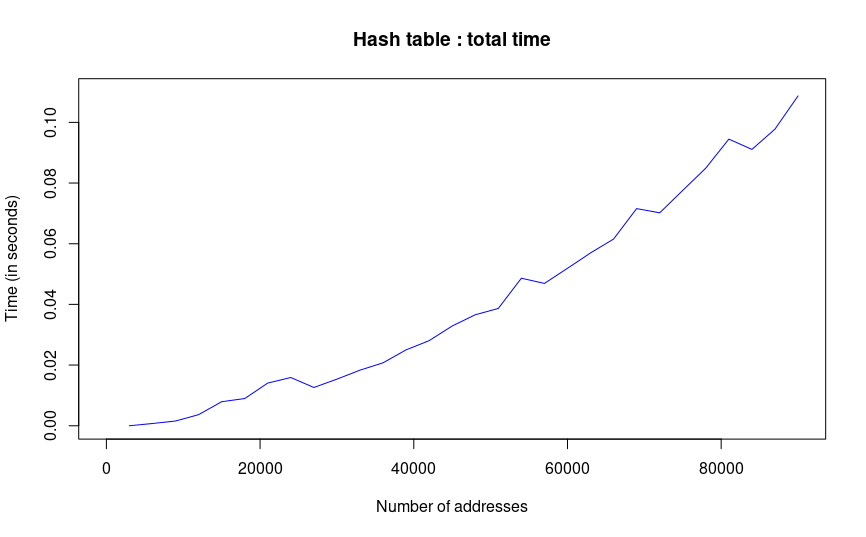
\includegraphics[scale=0.6]{plots/ht_total.png} 
  \caption{Total mean time passed in A.D.T. functions over 1000 tests according to the number of addresses stored in the structure.}\label{fig:ht}
\end{figure}
\subsubsection{Time passed in the MAGICindex function}
\paragraph{}We resumed the time passed in the \texttt{MAGICindex} function on the graphic represented on the \autoref{fig:ht_index}. 
\begin{figure}[H]
  \centering
  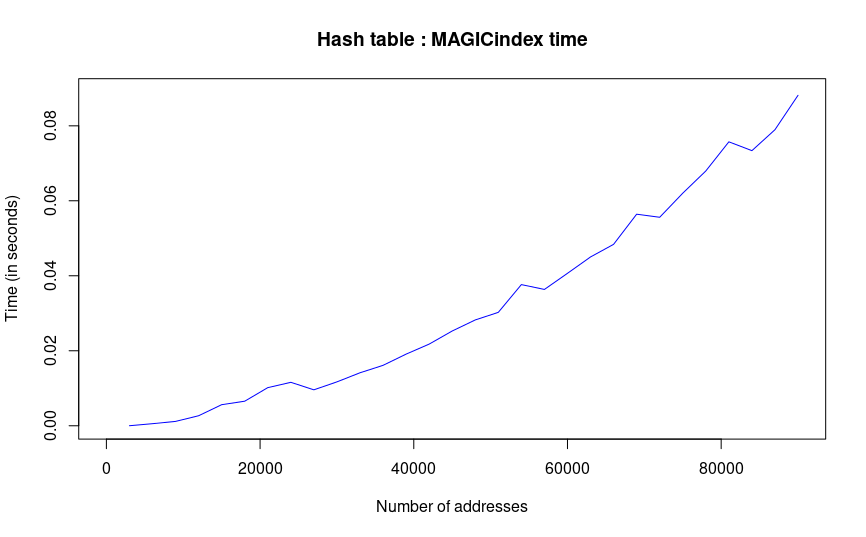
\includegraphics[scale=0.6]{plots/ht_index.png} 
  \caption{Mean time passed in the \texttt{MAGICindex} over 1000 tests according to the number of addresses stored in the structure.}\label{fig:ht_index}
\end{figure}
\subsubsection{Time passed in the MAGICreset function}
\paragraph{}We resumed the time passed in the \texttt{MAGICreset} function on the graphic represented on the \autoref{fig:ht_reset}. 
\begin{figure}[H]
  \centering
  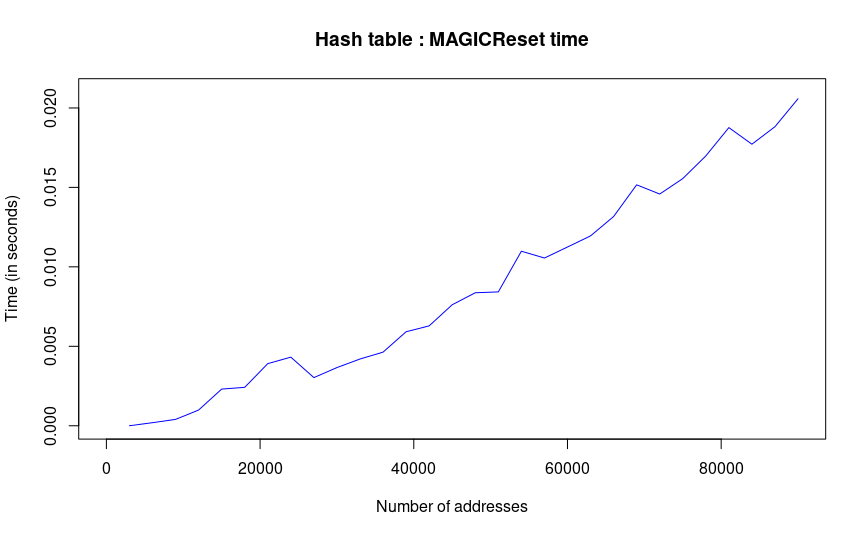
\includegraphics[scale=0.6]{plots/ht_reset.png} 
  \caption{Mean time passed in the \texttt{MAGICreset} over 1000 tests according to the number of addresses stored in the structure.}\label{fig:ht_reset}
\end{figure}

\subsection{Second implementation : Ternary search trie}
\paragraph{}We resumed the total time passed in the A.D.T. functions on the graphic represented on the \autoref{fig:tst}. 
\begin{figure}[H]
  \centering
  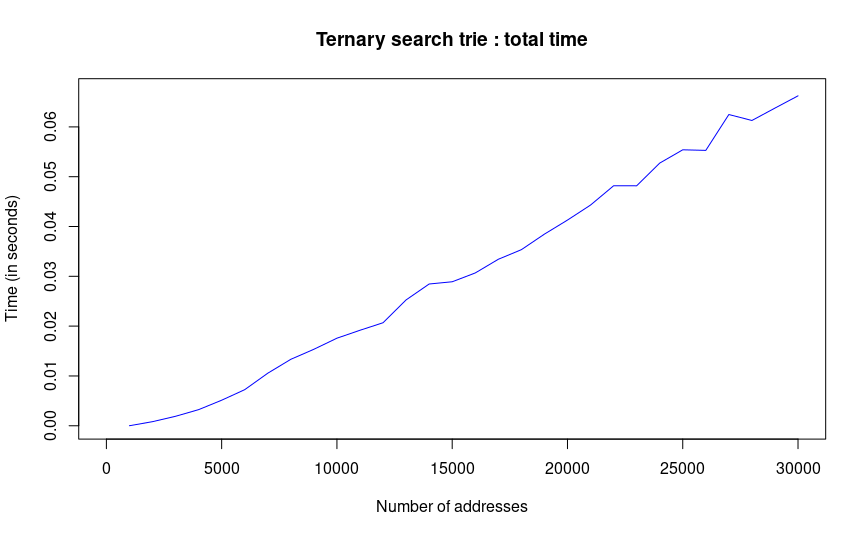
\includegraphics[scale=0.6]{plots/tst_total.png} 
  \caption{Total mean time passed in A.D.T. functions over 1000 tests according to the number of addresses stored in the structure.}\label{fig:tst}
\end{figure}
\subsubsection{Time passed in the MAGICindex function}
\paragraph{}We resumed the time passed in the \texttt{MAGICindex} function on the graphic represented on the \autoref{fig:tst_index}. 
\begin{figure}[H]
  \centering
  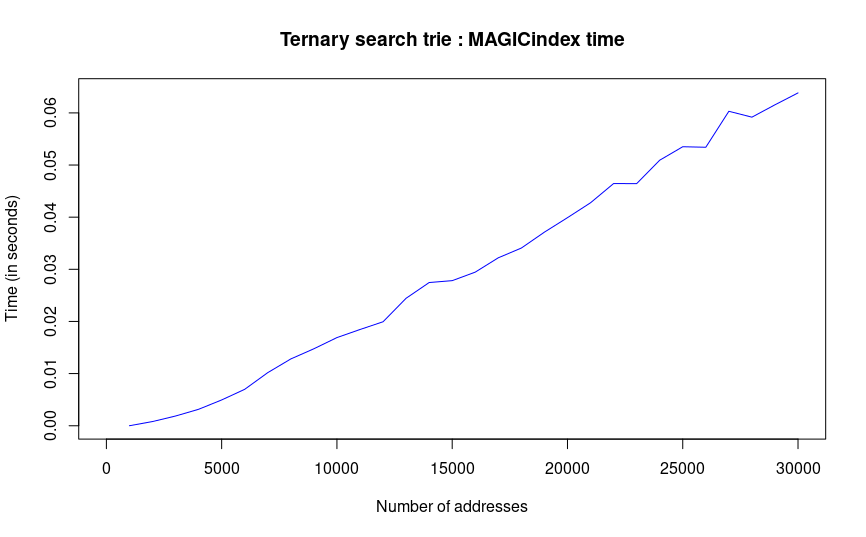
\includegraphics[scale=0.6]{plots/tst_index.png} 
  \caption{Mean time passed in the \texttt{MAGICindex} over 1000 tests according to the number of addresses stored in the structure.}\label{fig:tst_index}
\end{figure}
\subsubsection{Time passed in the MAGICreset function}
\paragraph{}We resumed the time passed in the \texttt{MAGICreset} function on the graphic represented on the \autoref{fig:tst_reset}. 
\begin{figure}[H]
  \centering
  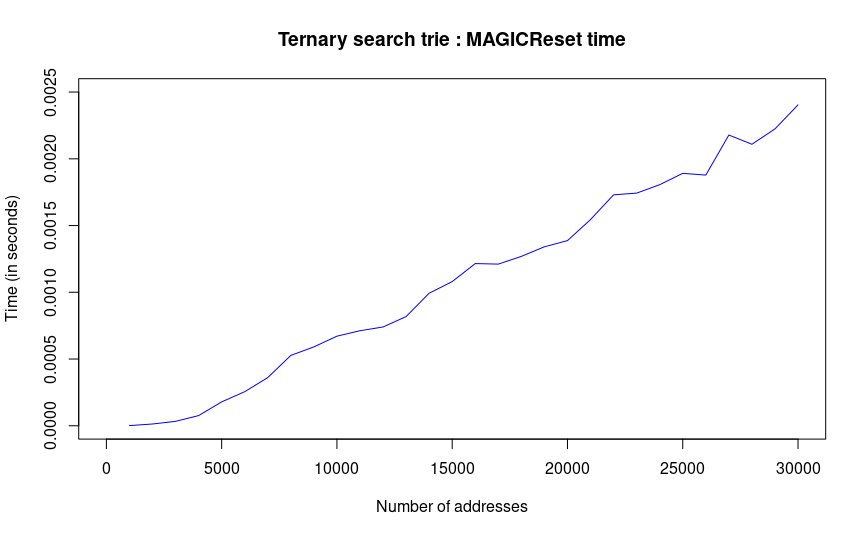
\includegraphics[scale=0.6]{plots/tst_reset.png} 
  \caption{Mean time passed in the \texttt{MAGICreset} over 1000 tests according to the number of addresses stored in the structure.}\label{fig:tst_reset}
\end{figure}

\subsection{Conclusion}
\paragraph{}Our first implementation (hash table) seems to have better perfomances than our second one (ternary search trie) in the \texttt{MAGICindex} implementation. However, our second implementation
has better performances in the \texttt{MAGICreset} implementation.

\paragraph{}In total, our first implementation seems to have better performances than our second one in terms of time.

\end{document}
